\documentclass[aspectratio=169,11pt]{beamer}

\usepackage[T1]{fontenc}
\usepackage[utf8]{inputenc}
\usepackage{lmodern}
\usepackage{array}
\usepackage{booktabs}
\usepackage{graphicx}
\usepackage{tikz}
\usetikzlibrary{positioning,arrows.meta,fit}

%% The deck shares the report's palette so the two read as one piece of
%% work: ink for structure, clay for anything the audience must not skim.
\definecolor{ink}{HTML}{1F3348}
\definecolor{clay}{HTML}{B4552D}
\definecolor{moss}{HTML}{3F6B52}
\definecolor{slate}{HTML}{4A5D78}
\definecolor{parchment}{HTML}{F4F1EA}
\definecolor{rule}{HTML}{C9C2B4}

%% A plain theme, built by hand. The stock beamer themes spend a third of
%% every slide on navigation furniture nobody clicks during a talk.
\usetheme{default}
\usecolortheme{default}
\setbeamertemplate{navigation symbols}{}
\setbeamercolor{structure}{fg=ink}
\setbeamercolor{frametitle}{fg=ink,bg=}
\setbeamercolor{normal text}{fg=ink}
\setbeamercolor{itemize item}{fg=clay}
\setbeamercolor{itemize subitem}{fg=slate}
\setbeamerfont{frametitle}{series=\bfseries,size=\large}
\setbeamerfont{framesubtitle}{size=\small,shape=\itshape}
\setbeamercolor{framesubtitle}{fg=slate}
\setbeamertemplate{itemize item}{\textbullet}
\setbeamertemplate{itemize subitem}{--}

%% A rule under the frame title, matching the report's section headings.
\setbeamertemplate{frametitle}{%
  \vskip0.6em%
  \usebeamerfont{frametitle}\usebeamercolor[fg]{frametitle}%
  \insertframetitle\par%
  \ifx\insertframesubtitle\@empty\else
    {\usebeamerfont{framesubtitle}\usebeamercolor[fg]{framesubtitle}%
     \insertframesubtitle\par}%
  \fi
  \vskip0.2em{\color{clay}\hrule height 1.2pt}\vskip0.4em}

%% Slide number in the corner, so the audience can cite one in questions.
%% Set in a filled chip so it stays legible over the tinted backdrop. The
%% chip is smashed to zero height: a taller footline steals vertical space
%% from the body and pushes the fullest slides into overfull boxes.
\setbeamertemplate{footline}{%
  \hfill\smash{\setlength{\fboxsep}{2.5pt}%
    \colorbox{ink}{\color{parchment}\scriptsize
      \insertframenumber/\inserttotalframenumber}}%
  \hspace{1.2em}\vskip0.9em}

%% ------------------------------------------------------------- backdrop
%% A white slide reads as a printed document and a heavy stock template
%% reads as a sales deck. This sits between the two: a warm near-white
%% page, the report's clay as a single accent down one edge, and a soft
%% wedge in the far corner for depth. The tint is kept very light so that
%% every text colour already chosen stays at full contrast, and so the
%% parchment panels still read as raised against it.
\newcommand{\bgplain}{%
  \begin{tikzpicture}[remember picture,overlay]
    \fill[parchment!40!white]
      (current page.south west) rectangle (current page.north east);
    \fill[ink]
      (current page.north west) rectangle
      ([yshift=-5pt]current page.north east);
    \fill[clay]
      ([yshift=-5pt]current page.north west) rectangle
      ([xshift=4pt]current page.south west);
    \fill[ink!7]
      ([xshift=-3.2cm]current page.south east) --
      (current page.south east) --
      ([yshift=3.2cm]current page.south east) -- cycle;
  \end{tikzpicture}}

%% The opening slide is the fullest one, so its variant adds depth with
%% two faint wedges rather than a solid band: a printed bar at the foot
%% would run underneath the list of names.
\newcommand{\bgtitle}{%
  \begin{tikzpicture}[remember picture,overlay]
    \fill[parchment!65!white]
      (current page.south west) rectangle (current page.north east);
    \fill[ink]
      (current page.north west) rectangle
      ([yshift=-5pt]current page.north east);
    \fill[clay]
      ([yshift=-5pt]current page.north west) rectangle
      ([xshift=4pt]current page.south west);
    \fill[ink!10]
      ([xshift=-5.0cm]current page.south east) --
      (current page.south east) --
      ([yshift=3.0cm]current page.south east) -- cycle;
    \fill[clay!10]
      (current page.south west) --
      ([xshift=4.2cm]current page.south west) --
      ([yshift=2.4cm]current page.south west) -- cycle;
  \end{tikzpicture}}

\newcommand{\eps}{\ensuremath{\varepsilon}}

%% A tinted panel for machine output and grammar dumps, so generated text
%% is never mistaken for prose. It is given a hairline edge because the
%% page behind it is no longer white.
\newcommand{\panel}[1]{%
  \begingroup\setlength{\fboxsep}{7pt}\setlength{\fboxrule}{0.4pt}%
  \noindent\fcolorbox{rule}{parchment}{%
    \begin{minipage}{\dimexpr\textwidth-16pt\relax}#1\end{minipage}}%
  \endgroup}

%% Screenshots. Missing files degrade to a labelled placeholder rather
%% than failing the build -- the same policy as the report.
\newcommand{\shot}[2]{%
  \setlength{\fboxsep}{0pt}\setlength{\fboxrule}{0.4pt}%
  \IfFileExists{screenshots/#1}
    {\fcolorbox{rule}{white}{\includegraphics[width=#2\linewidth]{screenshots/#1}}}
    {\IfFileExists{../screenshots/#1}
       {\fcolorbox{rule}{white}{\includegraphics[width=#2\linewidth]{../screenshots/#1}}}
       {\fcolorbox{rule}{parchment}{\begin{minipage}[c][3cm][c]{#2\linewidth}%
          \centering\small\color{clay}\itshape screenshot missing:\\
          {\ttfamily\footnotesize\upshape #1}\end{minipage}}}}}

\graphicspath{{./}{../}}

\begin{document}

\usebackgroundtemplate{\bgtitle}

\begin{frame}[plain]
\centering
\IfFileExists{ict-logo.jpg}
  {
\includegraphics[height=1.9cm]{ict-logo.jpg}}
  {\IfFileExists{../ict-logo.jpg}
     {
\includegraphics[height=1.9cm]{../ict-logo.jpg}}{}}
\\[0.5em]
{\color{rule}\rule{0.9\linewidth}{0.8pt}}\\[0.6em]
{\LARGE\bfseries\color{ink} Lexical and Syntactic Analysis\\[0.2em]
of Informal Urban Communication in Yaound\'e\par}
\vspace{0.4em}
{\color{rule}\rule{0.9\linewidth}{0.8pt}}\\[0.8em]
{\small\color{slate}CS4110 --- Compiler Construction\par}
\vspace{0.9em}
{\footnotesize Fru Chi Ehud Neba {\ttfamily\footnotesize ICTU20241812} \\ Daniel Victor {\ttfamily\footnotesize ICTU20241332} \\ Tchelibo Ayolo Sherrylle Claire {\ttfamily\footnotesize ICTU20241316} \\ Kefeyin Hariette Sela {\ttfamily\footnotesize ICTU20241471}\par}
\end{frame}

\usebackgroundtemplate{\bgplain}

\begin{frame}{The problem}{Why ordinary parsing techniques do not simply apply}
\begin{columns}[T,onlytextwidth]
\begin{column}{0.54\textwidth}
\begin{itemize}\setlength{\itemsep}{0.5em}
\item Everyday speech in Yaound\'e mixes French, English, Pidgin and Camfranglais {\bfseries inside a single sentence}.
\item Whitespace does not mark lexeme boundaries: {\ttfamily Carrefour Obili} is {\bfseries one} place name.
\item The same form changes grammatical class with context, which a lexer cannot see.
\item[] 
\item[{\color{clay}\bfseries Goal}] Apply the {\bfseries lexical} and {\bfseries syntactic} phases of a compiler to this register, and report honestly where they stop working.
\end{itemize}
\end{column}
\begin{column}{0.44\textwidth}
\panel{\small
\textbf{One corpus statement}\\[0.4em]
{\ttfamily Chef, drop me for Carrefour Obili.}\\[0.6em]
{\color{slate}\footnotesize
{\ttfamily Chef} --- French, used as a vocative\\
{\ttfamily drop} --- English verb, Pidgin sense\\
{\ttfamily for} --- Pidgin preposition, not English\\
{\ttfamily Carrefour Obili} --- one multiword lexeme\par}
}
\vspace{0.7em}
\footnotesize{\color{clay}15 of 15} collected statements draw on more than one language.
\end{column}
\end{columns}
\end{frame}

\begin{frame}{Method}{One pipeline, built and tested phase by phase}
\centering
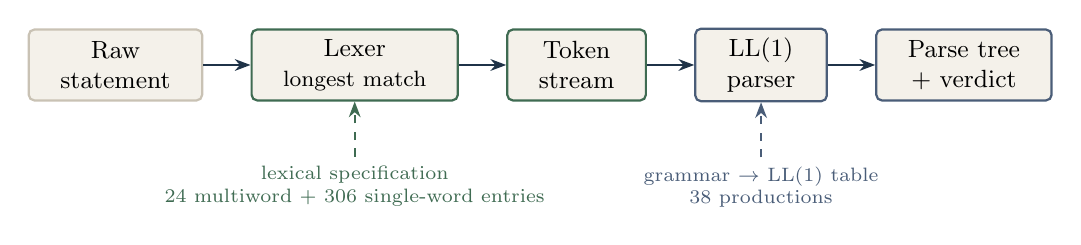
\begin{tikzpicture}[
  node distance=6mm,
  box/.style={draw=rule,line width=0.8pt,fill=parchment,rounded corners=2pt,minimum height=9mm,inner xsep=4mm,align=center,font=\small},
  lex/.style={box,draw=moss},
  syn/.style={box,draw=slate},
  arr/.style={-{Stealth[length=2mm]},draw=ink,line width=0.7pt}]
\node[box]            (src)  {Raw\\statement};
\node[lex,right=of src] (lex)  {Lexer\\{\footnotesize longest match}};
\node[lex,right=of lex] (tok)  {Token\\stream};
\node[syn,right=of tok] (par)  {LL(1)\\parser};
\node[syn,right=of par] (tree) {Parse tree\\+ verdict};
\draw[arr] (src) -- (lex);
\draw[arr] (lex) -- (tok);
\draw[arr] (tok) -- (par);
\draw[arr] (par) -- (tree);
\node[below=7mm of lex,font=\scriptsize,text=moss,align=center] (l1) {lexical specification\\24 multiword + 306 single-word entries};
\node[below=7mm of par,font=\scriptsize,text=slate,align=center] (l2) {grammar $\to$ LL(1) table\\38 productions};
\draw[arr,dashed,draw=moss] (l1) -- (lex);
\draw[arr,dashed,draw=slate] (l2) -- (par);
\end{tikzpicture}
\vspace{0.9em}
\begin{itemize}\setlength{\itemsep}{0.35em}
\item Corpus of {\color{clay}\bfseries 15} statements, plus {\color{clay}\bfseries 6} constructed counter-examples that {\itshape must} be rejected.
\item Unknown input is {\bfseries reported}, never silently dropped.
\end{itemize}
\end{frame}

\begin{frame}{Where this project sits}{A compiler has six phases; we build the first two, properly}
\centering
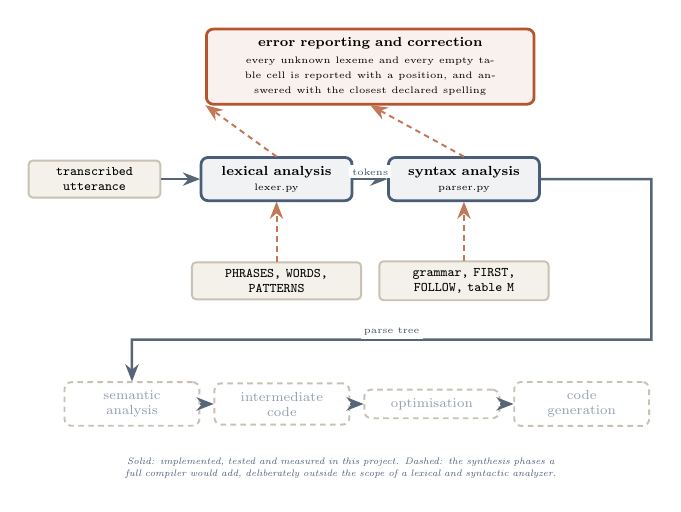
\begin{tikzpicture}[
  scale=0.68, transform shape,
  font=\small,
  >={Stealth[length=2.2mm,width=1.7mm]},
  state/.style={draw=ink, fill=white, line width=0.9pt,
                circle, minimum size=10mm, inner sep=0.3mm,
                align=center, font=\scriptsize\bfseries},
  probe/.style={draw=moss, fill=moss!8, line width=0.9pt,
                rounded corners=2.5pt, align=center,
                font=\scriptsize, inner sep=1.5mm},
  final/.style={draw=clay, fill=clay!10, line width=1pt,
                rounded corners=2.5pt, align=center,
                font=\scriptsize\bfseries, inner sep=1.5mm},
  box/.style={draw=rule, fill=parchment, line width=0.7pt,
              rounded corners=1.5pt, align=center,
              font=\scriptsize\ttfamily, inner sep=1.3mm},
  cell/.style={draw=rule, fill=white, line width=0.6pt,
               minimum width=9mm, minimum height=5mm,
               font=\tiny\ttfamily, inner sep=0.5mm},
  live/.style={draw=slate, fill=slate!8, line width=1pt,
               rounded corners=2.5pt, align=center,
               font=\scriptsize, inner sep=1.6mm},
  dead/.style={draw=rule, fill=white, line width=0.7pt,
               rounded corners=2.5pt, align=center,
               font=\scriptsize, inner sep=1.6mm,
               dash pattern=on 2pt off 1.6pt, text=slate!60},
  flow/.style={->, line width=0.9pt, draw=ink!75},
  back/.style={->, line width=0.7pt, draw=slate!70,
               dash pattern=on 2pt off 1.6pt},
  feed/.style={->, line width=0.7pt, draw=clay!80,
               dash pattern=on 2pt off 1.6pt},
  lab/.style={font=\tiny, inner sep=0.6mm, fill=white,
              text=ink!85, align=center},
  note/.style={font=\tiny\itshape, text=slate, align=center},
]
\node[box, text width=22mm] (src) at (0,0) {transcribed\\ utterance};
\node[live, text width=25mm] (lex) at (3.4,0)
  {\textbf{lexical analysis}\\ {\tiny lexer.py}};
\node[live, text width=25mm] (syn) at (6.9,0)
  {\textbf{syntax analysis}\\ {\tiny parser.py}};

\node[dead, text width=22mm] (sem) at (0.7,-4.2) {semantic\\ analysis};
\node[dead, text width=22mm] (ir)  at (3.5,-4.2) {intermediate\\ code};
\node[dead, text width=22mm] (opt) at (6.3,-4.2) {optimisation};
\node[dead, text width=22mm] (gen) at (9.1,-4.2) {code\\ generation};

\node[box, text width=29mm] (spec) at (3.4,-1.9)
  {PHRASES, WORDS,\\ PATTERNS};
\node[box, text width=29mm] (gram) at (6.9,-1.9)
  {grammar, FIRST,\\ FOLLOW, table M};

\node[live, text width=58mm, draw=clay, fill=clay!8] (err) at (5.15,2.1)
  {\textbf{error reporting and correction}\\[1pt]
   {\tiny every unknown lexeme and every empty table cell is reported with a
    position, and answered with the closest declared spelling}};

\draw[flow] (src) -- (lex);
\draw[flow] (lex) -- node[lab, above] {tokens} (syn);
\draw[flow] (sem) -- (ir);
\draw[flow] (ir) -- (opt);
\draw[flow] (opt) -- (gen);

\draw[flow] (syn.east) -- (10.4,0) -- (10.4,-3.0)
  -- node[lab, above] {parse tree} (0.7,-3.0) -- (sem.north);

\draw[feed] (spec.north) -- (lex.south);
\draw[feed] (gram.north) -- (syn.south);

\draw[feed] (lex.north) -- (err.south west);
\draw[feed] (syn.north) -- (err.south);

\node[note, text width=86mm] at (4.6,-5.4)
  {Solid: implemented, tested and measured in this project. Dashed: the
   synthesis phases a full compiler would add, deliberately outside the scope
   of a lexical and syntactic analyzer.};
\end{tikzpicture}
\vspace{0.3em}
{\footnotesize Analysis is implemented and measured. Synthesis is out of scope --- and saying so precisely is part of the answer.}
\end{frame}

\begin{frame}{Lexical analysis}{Longest match, with multiword lexemes tried first}
\begin{columns}[T,onlytextwidth]
\begin{column}{0.46\textwidth}
\begin{itemize}\setlength{\itemsep}{0.45em}
\item {\color{clay}\bfseries 24} multiword lexemes are matched {\itshape before} single words, so a compound is never split.
\item {\color{clay}\bfseries 306} single-word entries carry token type, source language, slang flag and gloss.
\item Spelling variation is folded to a normal form, so {\ttfamily wa} and {\ttfamily wah} count as one item.
\item Corpus yields {\color{clay}\bfseries 134} tokens over {\color{clay}\bfseries 76} distinct items.
\end{itemize}
\end{column}
\begin{column}{0.52\textwidth}
\panel{\scriptsize
\textbf{Chef, drop me for Carrefour Obili.}\\[0.5em]
\begin{tabular}{@{}r l l@{}}
\textbf{\#} & \textbf{lexeme} & \textbf{token}\\[0.2em]
1 & {\ttfamily Chef} & {\ttfamily VOC}\\
2 & {\ttfamily ,} & {\ttfamily SEP}\\
3 & {\ttfamily drop} & {\ttfamily VERB}\\
4 & {\ttfamily me} & {\ttfamily PRON}\\
5 & {\ttfamily for} & {\ttfamily PREP}\\
6 & {\ttfamily Carrefour} & {\ttfamily NOUN}\\
7 & {\ttfamily Obili} & {\ttfamily NOUN}\\
8 & {\ttfamily .} & {\ttfamily TERM}\\
\end{tabular}
\\[0.6em]
{\color{slate}token stream}\\
{\ttfamily VOC SEP VERB PRON PREP NOUN NOUN TERM \$}
}
\end{column}
\end{columns}
\end{frame}

\begin{frame}{The scanner as an automaton}{Three probes, tried in this order at every position}
\centering
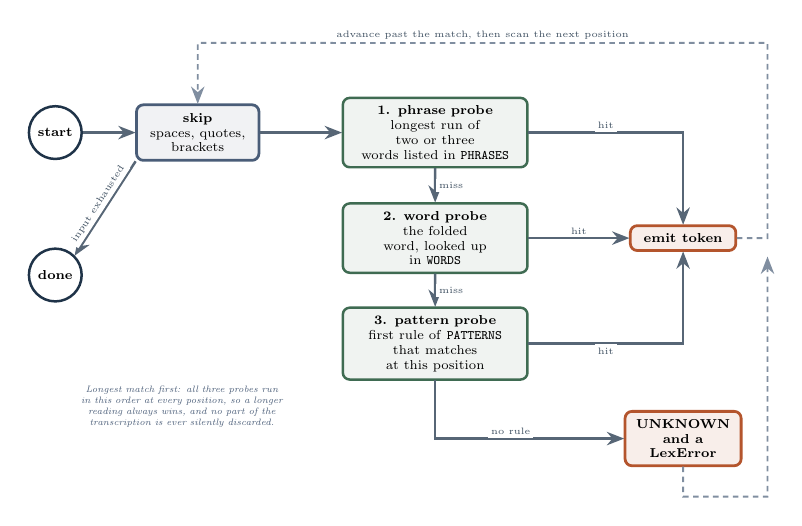
\begin{tikzpicture}[
  scale=0.67, transform shape,
  font=\small,
  >={Stealth[length=2.2mm,width=1.7mm]},
  state/.style={draw=ink, fill=white, line width=0.9pt,
                circle, minimum size=10mm, inner sep=0.3mm,
                align=center, font=\scriptsize\bfseries},
  probe/.style={draw=moss, fill=moss!8, line width=0.9pt,
                rounded corners=2.5pt, align=center,
                font=\scriptsize, inner sep=1.5mm},
  final/.style={draw=clay, fill=clay!10, line width=1pt,
                rounded corners=2.5pt, align=center,
                font=\scriptsize\bfseries, inner sep=1.5mm},
  box/.style={draw=rule, fill=parchment, line width=0.7pt,
              rounded corners=1.5pt, align=center,
              font=\scriptsize\ttfamily, inner sep=1.3mm},
  cell/.style={draw=rule, fill=white, line width=0.6pt,
               minimum width=9mm, minimum height=5mm,
               font=\tiny\ttfamily, inner sep=0.5mm},
  live/.style={draw=slate, fill=slate!8, line width=1pt,
               rounded corners=2.5pt, align=center,
               font=\scriptsize, inner sep=1.6mm},
  dead/.style={draw=rule, fill=white, line width=0.7pt,
               rounded corners=2.5pt, align=center,
               font=\scriptsize, inner sep=1.6mm,
               dash pattern=on 2pt off 1.6pt, text=slate!60},
  flow/.style={->, line width=0.9pt, draw=ink!75},
  back/.style={->, line width=0.7pt, draw=slate!70,
               dash pattern=on 2pt off 1.6pt},
  feed/.style={->, line width=0.7pt, draw=clay!80,
               dash pattern=on 2pt off 1.6pt},
  lab/.style={font=\tiny, inner sep=0.6mm, fill=white,
              text=ink!85, align=center},
  note/.style={font=\tiny\itshape, text=slate, align=center},
]
\node[state] (start) at (0,0) {start};
\node[live, text width=20mm] (skip) at (2.7,0)
  {\textbf{skip}\\ spaces, quotes,\\ brackets};

\node[probe, text width=32mm] (ph) at (7.2,0)
  {\textbf{1. phrase probe}\\ longest run of two or three\\
   words listed in \texttt{PHRASES}};
\node[probe, text width=32mm] (vo) at (7.2,-2.0)
  {\textbf{2. word probe}\\ the folded word, looked up\\
   in \texttt{WORDS}};
\node[probe, text width=32mm] (re) at (7.2,-4.0)
  {\textbf{3. pattern probe}\\ first rule of \texttt{PATTERNS}\\
   that matches at this position};

\node[final, text width=17mm] (emit) at (11.9,-2.0) {emit token};
\node[final, text width=19mm] (unk) at (11.9,-5.8)
  {UNKNOWN\\ and a LexError};

\node[state] (done) at (0,-2.7) {done};

\draw[flow] (start) -- (skip);
\draw[flow] (skip) -- (ph);

\draw[flow] (ph.east) -| node[lab, pos=0.25, above] {hit} (emit.north);
\draw[flow] (vo.east) -- node[lab, above] {hit} (emit.west);
\draw[flow] (re.east) -| node[lab, pos=0.25, below] {hit} (emit.south);

\draw[flow] (ph) -- node[lab, right] {miss} (vo);
\draw[flow] (vo) -- node[lab, right] {miss} (re);
\draw[flow] (re.south) |- node[lab, pos=0.7, above] {no rule} (unk.west);

\draw[back] (emit.east) -- (13.5,-2.0) -- (13.5,1.7)
  -- node[lab, above] {advance past the match, then scan the next position}
  (2.7,1.7) -- (skip.north);
\draw[back] (unk.south) -- (11.9,-6.9) -- (13.5,-6.9) -- (13.5,-2.35);

\draw[flow] (skip.south west) -- node[lab, sloped, above] {input exhausted}
  (done.north east);

\node[note, text width=42mm] at (2.4,-5.2)
  {Longest match first: all three probes run in this order at every
   position, so a longer reading always wins, and no part of the
   transcription is ever silently discarded.};
\end{tikzpicture}
\vspace{0.2em}
{\footnotesize The order {\itshape is} the specification: phrase before word, word before pattern. That is what makes {\ttfamily small small} one adverb.}
\end{frame}

\begin{frame}{From a natural grammar to an LL(1) one}{The grammar was written honestly first, then transformed}
\begin{columns}[T,onlytextwidth]
\begin{column}{0.5\textwidth}
{\small\color{clay}\bfseries 1. Remove left recursion}
\vspace{0.3em}
\panel{\scriptsize
{\ttfamily ClauseList} $\to$ {\ttfamily ClauseList SEP Clause}\\
{\ttfamily ClauseList} $\to$ {\ttfamily Clause}\\
\vspace{0.3em}{\color{clay}$\Downarrow$ immediate left recursion on ClauseList, introduced ClauseList'}\\[0.3em]
{\ttfamily ClauseList} $\to$ {\ttfamily Clause ClauseList'}\\
{\ttfamily ClauseList'} $\to$ {\ttfamily SEP Clause ClauseList'}\\
{\ttfamily ClauseList'} $\to$ {\ttfamily \eps{}}\\
}
\end{column}
\begin{column}{0.5\textwidth}
{\small\color{clay}\bfseries 2. Left-factor the common prefix}
\vspace{0.3em}
\panel{\scriptsize
{\ttfamily Clause} $\to$ {\ttfamily Subj VP}\\
{\ttfamily Clause} $\to$ {\ttfamily Subj COP Items}\\
\vspace{0.3em}{\color{clay}$\Downarrow$ common prefix 'Subj', introduced Clause\_f}\\[0.3em]
{\ttfamily Clause} $\to$ {\ttfamily Subj Clause\_f}\\
{\ttfamily Clause\_f} $\to$ {\ttfamily VP}\\
{\ttfamily Clause\_f} $\to$ {\ttfamily COP Items}\\
}
\end{column}
\end{columns}
\vspace{0.8em}
\footnotesize Both transformations are performed {\bfseries in code}, not by hand: {\ttfamily remove\_left\_recursion} and {\ttfamily left\_factor} run every time the analyzer starts, so the grammar shown and the grammar parsed cannot diverge.
\end{frame}

\begin{frame}{The LL(1) table --- and the one honest conflict}
\begin{columns}[T,onlytextwidth]
\begin{column}{0.48\textwidth}
\begin{itemize}\setlength{\itemsep}{0.45em}
\item FIRST and FOLLOW are computed to a fixed point, then the table is filled from them --- nothing is transcribed by hand.
\item {\color{clay}\bfseries 38} productions over {\color{clay}\bfseries 16} terminals.
\item An empty cell is a parse error, and the parser says {\itshape which} terminal it expected.
\end{itemize}
\end{column}
\begin{column}{0.5\textwidth}
\panel{\footnotesize
{\color{clay}\bfseries Conflict at M[NGopt, NOUN]}\\[0.4em]
After a noun phrase, a following NOUN could extend that phrase (Carrefour Obili as one name) or begin a new argument.\\[0.4em]
{\color{slate}This is a genuine ambiguity --- the dangling-else of this grammar. No rewriting removes it.}\\[0.4em]
{\bfseries Resolved} in favour of greedy compounding, which is the correct reading for every compound in the corpus.
}
\vspace{0.5em}
\footnotesize {\color{moss}\bfseries 0} undocumented conflicts. The one above is declared in the source and checked by a unit test, so it cannot be quietly forgotten.
\end{column}
\end{columns}
\end{frame}

\begin{frame}{The parser as a stack machine}{One token of lookahead, one stack, and a table that decides}
\centering
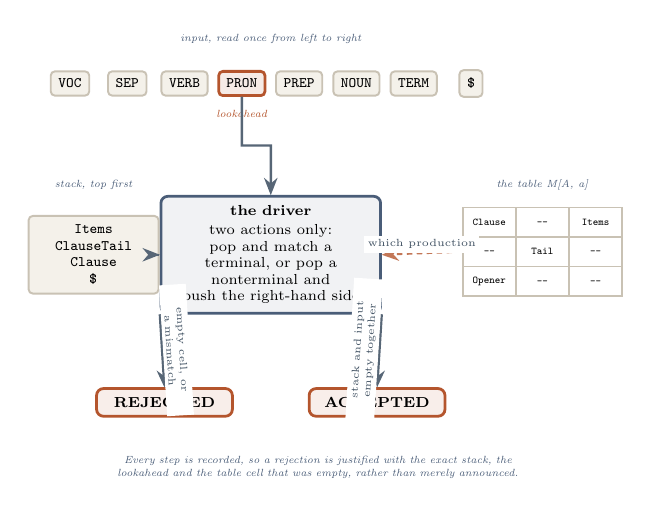
\begin{tikzpicture}[
  scale=0.75, transform shape,
  font=\small,
  >={Stealth[length=2.2mm,width=1.7mm]},
  state/.style={draw=ink, fill=white, line width=0.9pt,
                circle, minimum size=10mm, inner sep=0.3mm,
                align=center, font=\scriptsize\bfseries},
  probe/.style={draw=moss, fill=moss!8, line width=0.9pt,
                rounded corners=2.5pt, align=center,
                font=\scriptsize, inner sep=1.5mm},
  final/.style={draw=clay, fill=clay!10, line width=1pt,
                rounded corners=2.5pt, align=center,
                font=\scriptsize\bfseries, inner sep=1.5mm},
  box/.style={draw=rule, fill=parchment, line width=0.7pt,
              rounded corners=1.5pt, align=center,
              font=\scriptsize\ttfamily, inner sep=1.3mm},
  cell/.style={draw=rule, fill=white, line width=0.6pt,
               minimum width=9mm, minimum height=5mm,
               font=\tiny\ttfamily, inner sep=0.5mm},
  live/.style={draw=slate, fill=slate!8, line width=1pt,
               rounded corners=2.5pt, align=center,
               font=\scriptsize, inner sep=1.6mm},
  dead/.style={draw=rule, fill=white, line width=0.7pt,
               rounded corners=2.5pt, align=center,
               font=\scriptsize, inner sep=1.6mm,
               dash pattern=on 2pt off 1.6pt, text=slate!60},
  flow/.style={->, line width=0.9pt, draw=ink!75},
  back/.style={->, line width=0.7pt, draw=slate!70,
               dash pattern=on 2pt off 1.6pt},
  feed/.style={->, line width=0.7pt, draw=clay!80,
               dash pattern=on 2pt off 1.6pt},
  lab/.style={font=\tiny, inner sep=0.6mm, fill=white,
              text=ink!85, align=center},
  note/.style={font=\tiny\itshape, text=slate, align=center},
]
\node[note] at (3.4,0.75) {input, read once from left to right};

\node[box] (t1) at (0.00,0) {VOC};
\node[box] (t2) at (0.97,0) {SEP};
\node[box] (t3) at (1.94,0) {VERB};
\node[box, draw=clay, fill=clay!12, line width=1pt] (t4) at (2.91,0) {PRON};
\node[box] (t5) at (3.88,0) {PREP};
\node[box] (t6) at (4.85,0) {NOUN};
\node[box] (t7) at (5.82,0) {TERM};
\node[box] (t8) at (6.79,0) {\textdollar};

\node[note, text=clay] at (2.91,-0.52) {lookahead};

\node[live, text width=34mm] (ctrl) at (3.4,-2.9)
  {\textbf{the driver}\\[1pt]
   two actions only: pop and match a\\ terminal, or pop a nonterminal and\\
   push the right-hand side};

\node[box, text width=19mm, inner sep=1.5mm] (stk) at (0.4,-2.9)
  {Items\\ ClauseTail\\ Clause\\ \textdollar};
\node[note] at (0.4,-1.72) {stack, top first};

\node[cell] (m11) at (7.10,-2.35) {Clause};
\node[cell] (m12) at (8.00,-2.35) {--};
\node[cell] (m13) at (8.90,-2.35) {Items};
\node[cell] (m21) at (7.10,-2.85) {--};
\node[cell] (m22) at (8.00,-2.85) {Tail};
\node[cell] (m23) at (8.90,-2.85) {--};
\node[cell] (m31) at (7.10,-3.35) {Opener};
\node[cell] (m32) at (8.00,-3.35) {--};
\node[cell] (m33) at (8.90,-3.35) {--};
\node[note] at (8.00,-1.72) {the table M[A, a]};

\node[final, text width=20mm] (acc) at (5.2,-5.4) {ACCEPTED};
\node[final, text width=20mm] (rej) at (1.6,-5.4) {REJECTED};

\draw[flow] (t4.south) -- (2.91,-1.05) -- (3.4,-1.05) -- (ctrl.north);
\draw[flow] (stk.east) -- (ctrl.west);
\draw[feed] (m21.west) -- node[lab, above] {which production} (ctrl.east);

\draw[flow] (ctrl.south east) -- node[lab, sloped, above, text width=23mm]
  {stack and input empty together} (acc.north);
\draw[flow] (ctrl.south west) -- node[lab, sloped, above, text width=21mm]
  {empty cell, or a mismatch} (rej.north);

\node[note, text width=74mm] at (4.2,-6.5)
  {Every step is recorded, so a rejection is justified with the exact stack,
   the lookahead and the table cell that was empty, rather than merely
   announced.};
\end{tikzpicture}
\vspace{0.2em}
{\footnotesize The driver contains no grammar. Change the grammar and the table changes; the code does not.}
\end{frame}

\begin{frame}{Results}{Every acceptance carries a derivation; every rejection, a reason}
\begin{columns}[T,onlytextwidth]
\begin{column}{0.46\textwidth}
\panel{\footnotesize
\begin{tabular}{@{}l r@{}}
Statements collected & {\bfseries 15}\\
Accepted & {\color{moss}\bfseries 15}\\
Rejected & {\color{clay}\bfseries 0}\\
Counter-examples & {\bfseries 6}\\
Correctly rejected & {\color{moss}\bfseries 6}\\
Tokens & 134\\
Distinct items & 76\\
Type/token ratio & 56.7\%\\
\end{tabular}
}
\vspace{0.4em}
{\footnotesize\color{clay}\bfseries A rejection, with its reason}
\vspace{0.2em}
\shot{sets-panel.png}{0.88}
\end{column}
\begin{column}{0.52\textwidth}
{\footnotesize\color{clay}\bfseries FIRST and FOLLOW, computed at run time}
\vspace{0.25em}
\shot{trace-rejected.png}{0.84}
\vspace{0.35em}
\footnotesize The parser reports the stack, the remaining input and the terminal it expected --- not merely that the sentence failed.
\end{column}
\end{columns}
\end{frame}

\begin{frame}{The analyzer}{One engine, three front ends, live on the web}
\begin{columns}[T,onlytextwidth]
\begin{column}{0.62\textwidth}
\shot{app-overview.png}{0.96}
\end{column}
\begin{column}{0.36\textwidth}
\begin{itemize}\setlength{\itemsep}{0.35em}\small
\item All three front ends construct the {\bfseries same} {\ttfamily Analyzer}, so they cannot disagree about a verdict.
\item Tabs for tokens, tree, trace, derivation, FIRST/FOLLOW, corpus, statistics --- and {\bfseries Grammar}, which proposes a spelling when a word is rejected.
\item {\bfseries No third-party packages} --- the standard library only.
\item Deployed over HTTPS:
\item[] \raggedright{\ttfamily\tiny\color{clay} https://compiler-app.duckdns.org/}
\end{itemize}
\end{column}
\end{columns}
\end{frame}

\begin{frame}{What we found}{The interesting result is where the method stops}
\begin{columns}[T,onlytextwidth]
\begin{column}{0.49\textwidth}
{\small\color{moss}\bfseries What worked}
\begin{itemize}\setlength{\itemsep}{0.35em}\small
\item A restricted slice of the register is genuinely context-free and parses predictively.
\item Multiword lexemes solve compounding at the {\bfseries lexical} level, where it belongs.
\item Normalising spelling variants makes frequency counts meaningful across transcriptions.
\end{itemize}
\end{column}
\begin{column}{0.49\textwidth}
{\small\color{clay}\bfseries What did not}
\begin{itemize}\setlength{\itemsep}{0.35em}\small
\item Code-mixing operates {\bfseries below the clause}, sometimes inside a single lexeme --- a CFG cannot describe that.
\item Aspect is marked by free particles, not inflection, so the lexer cannot resolve class from form.
\item Noun compounding is {\bfseries genuinely ambiguous}; we document the resolution rather than hide it.
\item The corpus is transcribed by ear, without recordings.
\end{itemize}
\end{column}
\end{columns}
\end{frame}

\begin{frame}{Conclusion}
\begin{itemize}\setlength{\itemsep}{0.55em}
\item The lexical and syntactic phases of a compiler {\bfseries do} apply to informal Yaound\'e speech --- over a deliberately restricted grammar, with 15 of 15 statements accepted and all 6 counter-examples rejected.
\item Every number in this talk and in the report is {\bfseries computed}, not asserted: the same code that analyses the corpus writes the document and these slides.
\item The clearest next step is {\bfseries more data}, not more grammar. Replacing the corpus regenerates every table, figure and percentage automatically.
\end{itemize}
\vspace{0.6em}
\panel{\small\centering Try it: {\ttfamily\color{clay} https://compiler-app.duckdns.org/}\\[0.3em]{\footnotesize\color{slate}\ttfamily python -m yca web\quad$\cdot$\quad python -m yca test\quad$\cdot$\quad python -m yca report}}
\vspace{0.5em}
\centering{\color{ink}\large Thank you --- questions?}
\end{frame}

\end{document}
